\documentclass[30pt,twocolumn,letterpaper]{article}
\usepackage{cvpr}
\usepackage{times}
\usepackage{booktabs}
\usepackage{epsfig}
\usepackage{graphicx}
\usepackage{amsmath}
\usepackage{amssymb}
\cvprfinalcopy
\def\cvprPaperID{****}
\def\httilde{\mbox{\tt\raisebox{-.5ex}{\symbol{126}}}}
\usepackage{graphicx}
\usepackage{indentfirst}
\setlength{\parindent}{2em}
\usepackage{cite}
\usepackage[colorlinks,linkcolor=red,anchorcolor=blue,citecolor=green,backref=page]{hyperref}
\author{Qilei Zhang\\\\
Jun 16 2018}
\title{Fast and Accurate Recurrent Neural Network Acoustic Models for Speech Recognition}
\begin{document}
\maketitle
\begin{abstract}
  We have recently shown that deep Long Short-Term Memory (LSTM) recurrent neural networks (RNNs) outperform feed forward deep neural networks (DNNs) as acoustic models for speech recognition.
\end{abstract}
\section{Introduction}
While speech recognition systems using recurrent and feedforward neural networks have been around for more than two decades\cite{Barat2016String}, it is only recently that they have displaced Gaussian mixture models (GMMs) as the state-of-the-art acoustic model\cite{Eiber2013Attaining}. More recently, it has been shown that recurrent neural networks can outperform feed-forward networks on large-scale speech recognition tasks\cite{Krogh1995Neural}. \\
\begin{figure}[htbp]
\small
\centering
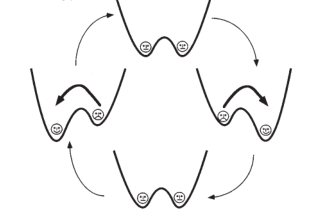
\includegraphics[width=20em]{000.png}
\caption{Layer connections in unidirectional (top) and bidirectional
(bottom) 5-layer LSTM RNNs.}
\label{fig:lable}
\end{figure}\\
\begin{equation}
\quad x'(t)=-V'(x)+A_0cos(wt+o)+u(t)
\end{equation}
\section{RNN Acoustic Modeling Techniques}
In this work we focus on the LSTM RNN architecture which has shown good performance in our previous research, outperforming deep neural networks.\cite{Pustejovsky1998The}.\\
\begin{figure}[htbp]
\small
\centering
\includegraphics[width=20em]{001.png}
\caption{Stacking and subsampling of frames. Acoustic features
are generated every 10ms, but are concatenated and downsampled
for input to the network: 8 frames are stacked for unidirectional
(top) and 3 for bidirectional models (bottom).
}
\label{fig:lable}
\end{figure}\\
\section{Experiments}
We train and evaluate LSTM RNN acoustic models on handtranscribed, anonymized utterances taken from real 16kHz Google voice search traffic\cite{Sanger1989Optimal}. Our training set consists of 3 million utterances with average duration of about 4s\cite{Szu1992Neural}. To achieve robustness to background noise and reverberant environments we synthetically distort each utterance in a room simulator with a virtual noise source\cite{Wittrock1989Generative}.
{\small
\bibliographystyle{ieee}
\bibliography{1}
}
\end{document}
